% SUDA_Courge_Project_Courge_Project
\documentclass[UTF8]{ctexart}
\usepackage{fancyhdr}
\usepackage{graphicx}
\usepackage{titlesec}
\usepackage{titletoc}
\usepackage{listings}
\usepackage{appendix}
\usepackage{bm, amsmath,amsfonts}
\usepackage{multirow}
\usepackage{tabularx}
\usepackage{setspace}
\usepackage{placeins}
% \usepackage{hyperref}
\usepackage{tcolorbox}
\usepackage{enumitem}
\tcbuselibrary{most}
\tcbuselibrary{skins, breakable, theorems}
% \usepackage{amsmath}
% \numberwithin{equation}{section}
\renewcommand{\theequation}{\arabic{section}-\arabic{equation}}


\usepackage[a4paper,left=3cm,right=3cm,top=3cm,bottom=2.54cm]{geometry}
\renewcommand{\contentsname}{\zihao{3} 目\quad 录}
\renewcommand{\abstractname}{\zihao{3} 摘\quad 要}

\counterwithin{figure}{section}

\makeatletter
\renewcommand{\thefigure}{\ifnum \c@section>\z@ \thesection-\fi \@arabic\c@figure}%章节与图片编号关联
\renewcommand{\thetable}{\ifnum \c@section>\z@ \thesection-\fi \@arabic\c@table}%章节与表格编号关联
\makeatother

\newtcolorbox{mybox}[2][]{colbacktitle=red!10!white, colback=blue!10!white,coltitle=red!70!black, title={#2},fonttitle=\bfseries,#1}

\newtcbtheorem{question}{题~(理}%
  {enhanced, breakable,
    colback = white, colframe = cyan, colbacktitle = cyan,
    attach boxed title to top left = {yshift = -2mm, xshift = 5mm},
    boxed title style = {sharp corners},
    fonttitle = \sffamily\bfseries, separator sign = {).~}}{qst}

 \newtcbtheorem[number within=section]{mytheo}{定理}%
  {colback=red!5,colframe=green!35!black,fonttitle=\bfseries}{th}

\lstdefinelanguage{HTML5}{
    sensitive=true,
    keywords={%
    % JavaScript
    typeof, new, true, false, catch, function, return, null, catch, switch, var, if, in, while, do, else, case, break,
    % HTML
    html, title, meta, style, head, body, script, canvas,
    % CSS
    border:, transform:, -moz-transform:, transition-duration:, transition-property:,
    transition-timing-function:
    },
    % http://texblog.org/tag/otherkeywords/
    otherkeywords={<, >, \/},   
    ndkeywords={class, export, boolean, throw, implements, import, this},   
    comment=[l]{//},
    % morecomment=[s][keywordstyle]{<}{>},  
    morecomment=[s]{/*}{*/},
    morecomment=[s]{<!}{>},
    morestring=[b]',
    morestring=[b]",    
    alsoletter={-},
    alsodigit={:}
}

% \ctexset{
%     % 修改 section。
%     section={ 
%     name={,、}
%         number={\arabic{section}},
%         format=\heiti\centering\zihao{3} % 设置 section 标题为黑体、居中对齐、3号字
%     },
%     % 修改 subsection。
%     subsection={
%     name={,、}
%         number={\arabic{subsection}},
%         format=\heiti\zihao{-3} % 设置 subsection 标题为黑体、5号字
%     },
%     % 修改 subsubsection。
%     % subsubsection={
%     % name={,、}
%     %     number={\arabic{subsubsection}},
%     %     format=\fangsong\zihao{-3} % 设置 subsection 标题为黑体、5号字
%     % }
% } 

%页眉页脚设置
\pagestyle{fancy}
\fancyhf{}
\cfoot{\thepage}
\chead{\songti\zihao{-5}{~宁波工程学院理学院学年论文~}}

%目录页设置
\titlecontents{section}[0em]{\zihao{4}\bf }{\thecontentslabel\ }{}
{\hspace{.5em}\titlerule*[4pt]{$\cdot$}\contentspage}
\titlecontents{subsection}[2em]{\vspace{0.1\baselineskip}\zihao{-4}}{\thecontentslabel\ }{}
{\hspace{.5em}\titlerule*[4pt]{$\cdot$}\contentspage}
\titlecontents{subsubsection}[4em]{\vspace{0.1\baselineskip}\zihao{-4}}{\thecontentslabel\ }{}
{\hspace{.5em}\titlerule*[4pt]{$\cdot$}\contentspage}
%代码设置
\RequirePackage{listings}
\RequirePackage{xcolor}
\definecolor{dkgreen}{rgb}{0,0.6,0}
\definecolor{gray}{rgb}{0.5,0.5,0.5}
\definecolor{mauve}{rgb}{0.58,0,0.82}
\lstset{
	numbers=left,  
	frame=tb,
	aboveskip=2mm,
	belowskip=2mm,
    breaklines=true,                 % automatic line breaking only at whitespace
	showstringspaces=false,
	columns=flexible,
	framerule=1pt,
	rulecolor=\color{gray!35},
	backgroundcolor=\color{gray!5},  % choose the background color
	basicstyle={\small},
	numberstyle=\tiny\color{gray},
	keywordstyle=\color{blue},       % keyword style
	commentstyle=\color{dkgreen},
	stringstyle=\color{mauve},
	breaklines=true,
	breakatwhitespace=true,
	tabsize=3,
    escapeinside={\%*}{*)},          % if you want to add LaTeX within your code
}
%------------------------------------------------------------------------
%正文部分
\setlength{\headheight}{13pt}
\pagenumbering{Roman}
\begin{document}
\zihao{-4}
	\begin{titlepage}
		\centering
		\vspace*{1.25cm}
        \quad
\includegraphics[width=0.8\linewidth]{figures/nbut_title.png}\\
        \vskip 1cm
        \fontsize{26pt}{0}{\heiti{理学院学年论文}}\\
        \vskip 1cm
        \quad
\includegraphics[width=0.3\linewidth]{figures/nbut_logo.eps}\\
        \vskip 1cm
		 \fontsize{16pt}{0}
		 \makebox[40mm]{论文(设计)题目:}
		 \underline{\makebox[100mm][c]{~基于居民区散点分布下~}}\\%在这里修改成自己的题目,题目太长写两行,英文和数学符号写在\Large{}里面
   	 \vskip 0.9cm
   	 \makebox[40mm]{}
		 \underline{\makebox[100mm][c]{~快递与同城配送站点的分析与研究~}}\\%第二行题目 \\
		 \vskip 0.9cm
		 \makebox[40mm]{专\hspace{7em} 业:}
		 \underline{\makebox[100mm][c]{~信息与计算科学~}}\\
		 \vskip 0.9cm
		 \makebox[40mm]{班\hspace{7em} 级:}
		 \underline{\makebox[100mm][c]{信科 \LARGE{19-1}}}\\
		 \vskip 0.9cm
		 \makebox[40mm]{姓\hspace{7em}名:}
		 \underline{\makebox[30mm][c]{岳云鹏}}
   	 \makebox[25mm]{学\hspace{2em} 号:}
		 \underline{\makebox[40mm][c]{ \LARGE 19480010103}}\\
		 \vskip 0.9cm
		 \makebox[40mm]{指\quad 导\quad 教\qquad 师:}
		 \underline{\makebox[30mm][c]{郭德纲}}
   	 \makebox[25mm]{职\hspace{2em} 称:}
		 \underline{\makebox[40mm][c]{副教授}}\\
		 \vskip 2cm
		 \Large \textbf{2022}~年~\textbf{6}~月~\textbf{17}~日	%指定日期
          %\Large \textbf{\number \year}~年~\textbf{\number \month}~月~\textbf{\number \day}~日
          %自动生成日期
	\end{titlepage}

 \begin{abstract}
 	% \pagestyle{plain}
        \pagestyle{fancy}
        \songti\zihao{-4}
  	% \thispagestyle{empty}   摘要页的页眉
\par 快递作为新兴行业,正改变人们的消费方式与生活习惯。快递派送工作,是配
送的最后一个环节。目前,快递派送阶段仍然采用以包裹分区承包设立的传统方式,主要存在快递派送区域规划不合理的问题。区域模糊K-Means聚类应用到区域划分中,实现区域规划的密度性合理优化,在快递区域派送中,为实现新的快递派送管理模式,运用算法规划最优派送路径,也能够对提高快递派送效率有较大意义。蚁群算法作为群智能算法的一种,能有效处理组合及聚类等优化问题。\rm{TSP}问题作为组合优化问题的代表,同时K-Means算法作为聚类问题的重要算法,近年来得到了广泛的研究。
\par 当前基于居民区的逐渐扩张,高楼大厦拔地而起。基于高密度的城市化进程中,散点分布的居民区是快递派送的主要目的地。基于对居民区的地理位置分析,希望规划出相对优化的快递站点的设立,便于居民和站点方便寄收快递的同时,为可能设立的快递临时收发点也有一定参考意义,基于此的考虑在区域快递问题上做出了本文的相关研究分析。同时在数据的展示上,制作对居民区的散点分布给读者可视化的图像界面,利用可视化技术将数据于图像融合展示,给读者更好的呈现。
\par 本文在研究居民区分布现状和快递派送现状及相关技术的基础上,对快递派送中存在的问题进行分析,并提出相应的解决规划。对快递派送最优区域划分和路径规划问题进行分析模拟,将其转化成散点图聚类问题和TSP旅行商问题,构建派送最优区域规划和路径规划的数学模型,利用蚁群算法找到相对的最优解,以在最优快递路径规划中的应用模型。
	\\[0.5cm]
	\textbf{关键字}:散点分布;K-Means聚类算法;TSP配送;区域划分;最优解
	\newpage
\end{abstract}

\tableofcontents
% \thispagestyle{empty}   目录页面的页眉

%\tableofcontents


% 第一章节、绪论
\clearpage
\pagenumbering{arabic}
\setcounter{page}{1}
\setcounter{equation}{0}
\section{绪 \quad 论}
\songti\zihao{-4}
\setlength{\baselineskip}{20pt}
\par 2020年,第十一届中国电子商务物流大会提出,”作为重要的基础行业,物流业在保障民生、促进经济社会良好运行、保证全球供应链的稳定方面发挥了重要作用”。当疫情席卷全球时,得益于我国电子商务和快递业的蓬勃发展及相关基础设施的完善,人们可以在避免密切接触的前提下获取所购买的商品,这种购物方式很大程度上保障了基本的安全需求和生活需求,也有利于疫情期间经济的恢复和社会秩序的稳定。国家邮政局数据显示,我国快递行业在2007年至2020年间实现了飞跃式的增长,快递业务量和快递业务收入分别从$2.29$亿件和$520$亿元增长至833.6亿件和8795.4亿元$^{[1]}$。
\par 快递行业近年来受到电子商务发展的影响,进入了快速发展的阶段。国内快递行业也逐渐变得百家争鸣。快递行业的发展同时也推动了互联网经济,促进劳动力就业,快递行业作为日常基础的服务行业日益受到人们的关注。 但目前快递配送“最后一公里”—快递派送,却成为了我国快递发展的瓶颈,经测算,快递在最后一公里的成本占比能达整个快递配送成本的50\%。[5]快递派送的服务质量和效率直接影响物流企业的发展。目前,快递员从营业网点出发执行派送任务,再回到营业网点,其派送路线的选择大多依赖主观经验,对于路线不熟悉缺乏了解,便会造成对派送业务和效率的影响。通过对派送路线的合理规划可以减少派送时间及运营成本,因此目前的人工派送或对未来的无人派送,都需要对派送路线和区域进行合理的规划。\cite{knuthwebsite} 若能利用数学的优势来解决快递派送过程中存在的问题,将有效提高快递企业资源利用率,降低企业运营成本,提高快递派送的效率,进而增强企业市场竞争力。这也将是本课题所要研究和探讨的主要问题,并提出自己的解决方案 \footnote{这是测试文字}。

\subsection{选题背景和研究现状}
\par 随着我国经济贸易持续繁荣发展,中国老字号的邮政的业务服务已经不能完全满足人民的需求,趋于全国物流运营规模的逐渐扩大和交通运输的便利发展,同城配送、异地运输、港澳台及国际快递等业务的逐渐开展,快递已然逐渐发展成为一个新兴的行业。形成了民营与国有企业共同发展竞争的形式。在一方面带来了便利,同时也推动了国家社会的经济发展。由于日前国家地区经济的不断发展,已知城市化的发展促使的交通运输的日益便利、经济日渐繁荣使得人民对物流的需求和要求的提高以及网络贸易迅速普及并急需构建出上线下便捷统一的高效服务,经济的快速发展使得对物流广大需求和更高要求使得快递行业日新月异逐渐成熟。快递业作为基础服务业之一,具有解决地域差异、加快实物传递、信息实时跟踪等多种重要功能,涉及交通运输、基础建设、信息技术、金融投资等多个行业的参与,是邮政业务中不可替代的重要组成部分。伴随着近年来网络贸易的繁荣和电子商务行业转型升级的需要,对快递业的服务能力要求进一步提升。\cite{dirac}
\par 在当前网络贸易经济繁荣茂盛下,大力促进了快递行业的发展并对快递行业有更高的要求。网络购物和网上支付的快速普及,快递业逐渐成为最贴近人们日常生活的产业之一,为大量社会经济活动和个人活动提供了基础的物品运输服务,快递需求日渐增加。快递行业作为经济贸易与交通迅速发展而诞生的新兴产业,优化快递配送为满足居民和顾客的需求和服务是如今的重要研究目标。
如今,快递行业通过近些年的快速发展,在港澳台及国际物流、异地物流、同城派送、生活服务类外卖、跑腿等上有巨大的业务拓展。近年来的迅猛发展使得快递物流配送行业社会话及专业化的趋势,为解决用户对快递的要求以及运营成本的影响增加问题,本文采用聚类规划区域并通过进一步聚类确立可能的分区域点并模拟规划区域配送路线求取最优解。\cite{knuth-fa}


\subsection{研究现状}
\par 快递派送管理,国际上有很多做法,常规的做法是先做零售,当网点布局到一定程度后,再借力网点做快递业务。譬如,在日本,便利店的快递收发功能已非常成熟,人们习惯于到距离家或者公司最近的便利店收发物件,顺便购买一些日用品。由于国情不同,我国在快递派送阶段采取的是基于人工收送货的直接配送模式,国内大多企业对于快递派送的管理依然采用以结果管理过程的传统方式,信息技术的应用较少[3]。 \cite{einstein}
我国快递行业因电子商务而快速发展,近年来发展势头迅猛。高度专业化和社会化是快递行业发展的趋势,营业网点作为快速最末端的服务点,承担着收取快件和派送快件的功能,而派送环节是快递十分重要的一个环节。[5]由于受传统思维的影响,行业内的许多企业的重心依然放在快递物流的运输配送过程中,即跨区域的物流周转,运用大量的先进技术来提高该过程的效率,但随着派送环节发展滞后对用户服务满意度以及运营成本的影响比重增加,行业内开始逐渐提高快递派送管理的重视。
\par 丁浩等研究快递车辆在运输过程中的最短路径选择问题,分别对车辆的最短路径使用遗传算法、A*算法、蚁群算法进行计算并与Dijkstra算法进行对比,结果证明合理的运用Dijkstra算法可以帮助快递企业寻找到最优路径从而降低运输成本;杨从平等针对不同配送路径会影响配送成本的情况,构建基于蚁群算法的快递车辆配送路径优化模型,并通过规则优化后的蚁群算法模型对广西省桂林市的某快递配送网络进行路径优化;宋娟等基于改进遗传算法的同城快递配送模型;倪霖等研究城市快递配送中的路径优化问题,在对多家快递企业共同配送的路径进行模拟分析后,发现快递车辆的装载率对配送效率有较大影响,据此使用改进的遗传算法对装载率与车辆油耗的数学模型进行求解,并对快递同时取送、共同配送、独立配送三种情况的车辆路径进行分别优化。

\subsection{研究的内容和解决问题}
\par 本文将以快递派送中存在的问题为切入点,围绕聚类划分和网络路径规划的区域派送最优路径规划进行展开。对区域聚类划分和派送最优路径问题进行多方研究和分析,将其转化为数学模型,然后运用K-Means聚类算法求解快递区域派送区域进一步规划局部路径。

\subsection{论文的组织结构}
\par 本文共分为五章,各章的内容如下: 
\begin{itemize}
    \item 第一章,绪论。介绍论文研究课题的研究背景和意义,当前存在的问题、课题的相关研究现状以及研究目的。
    \item 第二章,相关技术分析及选择。主要包括对散点数据处理、聚类算法问题的理论分析以及技术选择。
    \item  第三章,模糊聚类算法对散点数据的处理,改善了\rm{K-Means}算法的部分缺点,可以在无基础中心点下进行优化的判断中心点,减少选点带来的误差损失,对数据进行可视化表现为图像。
    \item 第四章,基于MTSP和改进算法TSP的对区域快递派送的划分后的处理,使派件在局部找到最优解问题。
    \item 第五章,总结和展望,对问题的小结以及改进内容。
\end{itemize}

% 第二章节、引言
\clearpage
\section{散点数据的处理和方法介绍}
\subsection{散点数据的处理}
\par 数据作为多种维度的信息,在数据表现上主要依靠图表展示。而散点图的数据分析方法主要是基于数值层面的方法、基于形状模式的方法、基于人对散点图的感知情况的方法。在数据展示的可视化处理上,比如散点图矩阵,就是将二维散点图进行重复排列,用户很容易理解。但当维数增多时,大量的散点图需要一定的展示空间,而且其数据分布也不容易被用户观察到。因此,许多工作着眼于识别大量散点图中用户感兴趣的散点图子集,并将子集呈现给用户。
\begin{table}[!ht]
    \centering
        \caption{各地域的经纬度地址}
    \begin{tabular}{ccccccccc}
    \hline
       区县  &  杭州市 &	上城区	& 下城区 &	江干区 & 拱墅区 & 西湖区	& 滨江区	& 萧山区\\ \hline
       经度  &  120.15 &	120.17	& 120.17 &	120.2 & 120.13 & 120.13	& 120.2	& 120.27 \\ 
       纬度  & 30.28  &	30.25	& 30.28 &	30.27 & 30.32 & 30.27	& 30.2	& 30.17 \\ \hline
    \end{tabular}
    \label{tab:my_label}
\end{table}

\begin{table}[!ht]
    \centering
     \caption{各地域的经纬度地址}
    \begin{tabular}{ccccccccc}
    \hline
       区县  &  余杭区 &	...	& 桐庐县 &	淳安县 & 建德市 & 富阳市	& 临安市	& 宁波市\\ \hline
       经度  &  120.3 &	...	& 119.67 &	119.03 & 119.28 & 119.95	& 119.72	& 121.55 \\ 
       纬度  & 30.42  &	...	& 29.8 &	29.67 & 29.48 & 30.05	& 30.23	& 29.88 \\ \hline
    \end{tabular}
    \label{tab:my_label}
\end{table}

\par 在地域的分类划分聚类中,就采用先呈现子集并聚类后分析的方法。如图2-1浙江省县市中心的地域分布图。

\begin{figure}[!ht]
    \centering
     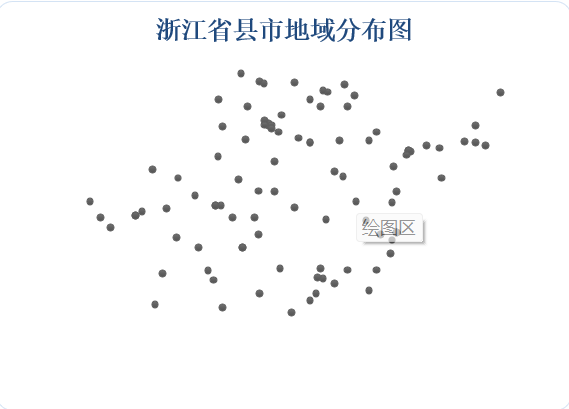
\includegraphics[width=0.5\textwidth]{fig2/fig21.png}
      \caption{浙江省县市中心的地域分布图}
\end{figure}
\FloatBarrier  %禁止图片浮动

\subsection{\rm{K-Means}聚类算法}
\subsubsection{算法简介}
\par K-Means算法(也叫$k$均值或$k$平均算法),是机器学习领域常见的一种无监督学习模型,其将距离作为相似性评价指标。在K-Means算法中,将距离较近的同类数据点放入一个簇内,且它们之间的距离应尽可能地接近;而不同簇的中心距离则应尽可能地远。
K-Means是一种广泛应用于配送网络末端配送区域划分的聚类算法。本文使用的算法根据预设的$m$个聚类中心对样本点进行聚类划分后,根据得到的每个类中点的平均值重新作为下次聚类划分的聚类中心,不断重复聚类划分的过程直到聚类中心不再发生变化,算法终止输出最优聚类结果。算法的目标是使聚类结果各类中的点尽可能的紧凑,并且使不同类别之间相互分开。

\subsubsection{算法过程}
\par 对数据进行基本处理后,计算其中各点的均值:

\begin{equation}
    \overline{x_i} = \frac{1}{n}\sum_{i=1}^na_{ij}
\end{equation}
\par 计算各个数据的具体的相对中心点的的位置:
 \begin{equation}
    z_i=\sqrt{\frac{1}{n-1}\sum_{i=1}^n(a_{ij}-\overline{x_i})^2}
\end{equation}
\par 计算出各个样本点两两之间的距离,并构造距离矩阵$(_{ik})_{n \times n}$ 。采用欧几里得距离:
 
\begin{equation}
    d_{ik} = \sqrt{\sum_{j=1}^m(z_{ij}-z_{kj})^2}
\end{equation}
\par 构造$n$个类且每个类只包含一个样本点,每一个类的平台高度为零。再合并距离最近的两类为新类,且这两类之间的距离值作为聚类图中的平台高度。最后,绘制出聚类图,选择所需要的决定类的个数和类。由于算法在聚类时需要先进行聚类中心的初始化,所以会导致聚类的不稳定;又因为每次迭代前都需要重新计算聚类中心,也增加了算法的时间复杂度。针对以上问题,所以采用模糊聚类的算法进行改进。

\subsection{模糊K-Means聚类算法}
\par 在K-Means算法下,每一个数据点$x$在分类时,均会被严格地放入某一个类别中。但在实际的分类过程中,这一个数据点$x$却难以严格地被划分到同一个类别中,其可能是以不同的隶属度划分到某一类。此时,对每一个分类结果均可用一个模糊分类矩阵表示:

\begin{equation}
U=\begin{bmatrix}
u_{11} & u_{12} & \cdots & u_{1n}\\
u_{21} & u_{22} & \cdots & u_{2n} \\
\vdots  & \vdots  & \ddots  &\vdots  \\
u_{c1} & u_{c2} & \cdots & u_{cn} \\
\end{bmatrix}
\end{equation}

\par 其中,$u_{ij} \in [0,1]$ 表示某个数据点对于该类别的隶属度。定义模糊分类下的误差平方准则函数为:
\begin{equation}
I_{m}=\sum_{i=1}^{c} \sum_{j=1}^{n} u_{i j}^{i m}\left\|\left|x_{j}-w_{i} \|\right|^{2}\right.
\end{equation}

\par 在计算聚类中心时,也需要进行模糊化处理:
\begin{equation}
    w_{i}(t)=\frac{\sum_{j=1}^{n}u_{ij}^{m}x_{j}}{\sum_{j=1}^{n}u_{ij}}
\end{equation}
在迭代过程中,需要对模糊矩阵进行修正,直至最后得出结果:
 
\begin{equation}
    u_{ij}(t+1) = \frac{1}{\sum_{i=1}^{c} (\left \| \left | \frac{x_{j}-w_{j}  }{x_{j}-w_{i}}  \right |  \right \| )^{\frac{z}{m-i}}} 
    \end{equation}
\subsection{散点分布的可视化}
\par 为了协助人们对数据的分析,将分析结果可视化是重要的。在清晰表达信息给读者时,在二维图像上能够提供更直观的信息表现。由于信息的数据反映在很大程度上取决于了表达方式,所以在分析由数字和列表组成的数据时。数据可视化的本质是展现数据,数据可视化是以图形的方式清晰有效地传达和传播信息。赋予了可视化数据的价值,帮助读者更好的从信息中提取,从图像中收获价值。
其中JavaScript语言可以对收集到的数据中的经纬度进行坐标映射转换为地图中的对应坐标值。再通过自建函数调用参数处理传入的参数数据,进而绘制出最后的结果。

\subsection{TSP算法}
\par 意大利学者\rm{Dorigo}等人提出了第一个蚁群算法—蚂蚁系统,并用于\rm{TSP}问题的求解。由于每只蚂蚁都可通过一种称为信息素的媒介来交流信息,指导自己选择下一步所要行走的路径。蚂蚁在行走过程中会在路径上释放信息素,因此每条路径都会被信息素所标记,蚂蚁可以检测信息素浓度,并以一定的概率朝着信息素浓度高的地方移动。这是一种正反馈机制,越多的蚂蚁选择相同的路径,则这条路径被选择的概率就越高,吸引更多的蚂蚁选择相同的路径,最终蚂蚁往返于巢穴到食物源间的最短路径。
\par 经过大量学者进行不断的优化,使\rm{Shelokar}将蚁群算法成功应用于求解聚类问题,从此开始了蚁群算法在聚类问题的应用。蚁群算法具有分布计算、信息正反馈和启发式搜索的特征,本质上是进化算法中的一种启发式全局优化算法。但是其在解决大型优化问题时,存在搜索空间和时间性能上的矛盾,易出现过早收敛于非全局最优解以及计算时间过长的弱点。近年来,依据蚁群算法求解问题的基本模型和流程,为能够加快蚁群算法收敛速度、提高算法的运行性能、避免局部最优和提高全局搜索能力等,主要的改进策略主要有三方面:蚁群算法的信息素更新策略改进、路径的选择策略改进、蚁群算法与其他算法的融合。由于蚁群算法模型会随着问题变化而略有改动,因此这一部分以求解TSP问题为线索介绍蚂蚁系统。

% 第三章节、主体
\clearpage
\setcounter{equation}{0}
\section{模糊聚类算法划分居民区域}
\subsection{区域划分聚类步骤}
为提高配送站点的配送效率,前提是要合理划分同城配送区域,确定最集中的配送中心点。

\begin{enumerate}
    \item 选择\rm{k}个初始中心点,例如\rm{c[0]=data[0]}, $\cdots$ \rm{c[k-1]=data[k-1]};
    \item 对于$data[0]$ $\cdots$ $data[n]$, 分别与$c[0]$ $\cdots$ $c[k-1]$比较,假定与$c[i]$差值最少,就标记为$i$;
    \item 对于所有标记为$i$点,重新计算$c[i]=$ \{所有标记为$i$的$data[j]$之和\}标记为$i$的个数;
    \item 重复(2)(3),直到所有$c[i]$值的变化小于给定阈值。
\end{enumerate}

K-Means算法简单易行、便于理解和操作,不但能够处理大规模的聚类问题,对本文研究的同城配送区域划分也有很好的应用效果。算法的聚类数k可以根据经验设定,也可以根据聚类分析对象的数据特征来设置。根据初次聚类的结果进行迭代更新,通过不断的迭代使结果不断接近判断标准,最终聚类结果达到目标标准,聚类中心不再发生变化,算法停止输出结果。

 \begin{figure}[h]
     \centering
     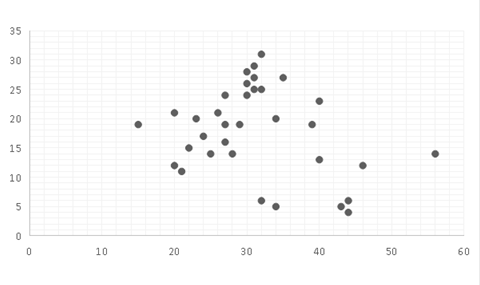
\includegraphics[width=0.5\textwidth]{fig3/fig31.png}
     \caption{居民区的散点分布经经纬度标准化后的散点图}
     \label{fig:my_label}
 \end{figure}
\FloatBarrier
\subsection{居民点的区域划分模型}
\par 本文将案例中需求点的经纬度信息转化为平面坐标,便于使用\rm{K-Means}算法进行求解。用需求点之间距离的大小代表不同需求点之间的相似性,距离越小代表相似性越大。将不同需求点之间的相似性作为划分配送区域的依据,将相似性大的需求点划分到同一个配送区域。为方便后续使用遗传算法对配送路径优化模型进行求解,将地理位置的经纬度信息转化为平面坐标。

\begin{figure}[h]
     \centering
     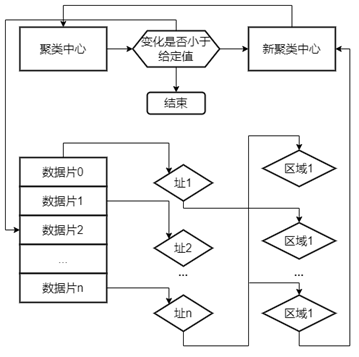
\includegraphics[width=0.5\textwidth]{fig3/fig32.png}
     \caption{K-means算法流程}
     \label{fig:my_label}
 \end{figure}
\FloatBarrier
算法的运行时间随着节点数量的变大而不断减小,这说明对模糊K-Means的并行化切实提升了算法的运行速度,算法具有较好的扩展性。通过模糊K-Means算法根据需求点的实际位置对配送区域进行划分,对聚类效果进行评价确定最佳聚类数为$n$,将$k$值设定为$n$,将配送区域化分为若干部分。

\begin{figure}[h]
     \centering
     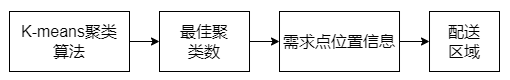
\includegraphics[width=0.5\textwidth]{fig3/fig33.png}
     \caption{K-means算法求解最佳配送区域过程}
     \label{fig:my_label}
 \end{figure}
\FloatBarrier
采用模糊K-Means聚类算法,根据订单需求点的地理位置,确定最佳聚类数,将订单划分到不同的配送区域,得到满足实际配送要求的最佳聚类结果。

\subsection{居民点的区域可视化}
根据上面所述,对区县中的居民点的散点进行统一整合。如下图3-4宁波市各个区县级的地域分布图。其中图中红色、蓝色、绿色区域分别表示鄞州区、海曙区和江北区,灰色区域表示其他区县地区。
\begin{figure}[h]
     \centering
     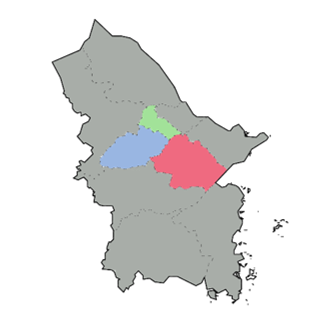
\includegraphics[width=0.3\textwidth]{fig3/fig34.png}
     \caption{宁波地理位置分布图}
     \label{fig:my_label}
\end{figure}
\FloatBarrier
  
根据数据进行统计对区县中的居民点的散点进行分析地址统计,整合出大概地址后,可在地图上二维呈现出散点图状。如下图3-5宁波市中心部分居民区散点分布图。其中由于小区居民散点过多,显示的红点为主要的大集中居民区点。
\begin{figure}[h]
     \centering
     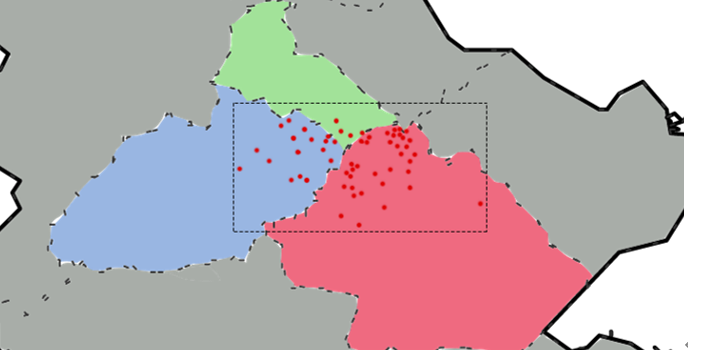
\includegraphics[width=0.5\textwidth]{fig3/fig35.png}
     \caption{宁波市中心部分居民区散点分布图}
     \label{fig:my_label}
\end{figure}
\FloatBarrier
 同时将居民点位置提取出来后,对居民点的具体地址的经纬度进行标准化等处理后,将便可对居民区的位置进行后续分析。


% 第四章节
\clearpage
\section{宁波居民区散点分布模型研究同城配送的模式和特性}
由于顾客多是散点状分布,这里涉及分组离散的网络图论问题。在确定派送策略时,我们可以通过合理的假设,将其转化为MTSP问题,因MTSP问题求解难度较大,可把MTSP问题转化为TSP问题解决,即可求出总的最短送货路程。以此最短路程为限制条件,利用基于最小生成树的深度优先搜索算法寻找合适的运行路线,并结合实际情况中的载重限制,对找出的运行路线进行调整修正,即可得出符合要求的运行路线。 
(下面利用TSP的蚁群算法的相关理论对问题进行分析。)

\subsection{MTSP算法模型}
给定$n$个城市($V_1$,$V_2$,…,$V_n$),$m$名旅行商皆以城市$V_0$为起点。令$W_{ij}$表示$V_i$城到$V_j$城的距离。

 $\Phi_{k}=(\nu_{i1},\nu_{i2},\nu_{i3},...,\nu_{in}$ ) 表示一条巡回路线。$\omega  (\Phi_{k})=(W_{i1},W_{i2},W_{i3},...,W_{in}$ 为$\Phi_{k}$巡回的总路程。目标是选择$m$条巡回路线使总路程最小,目标函数如下: 
 $\omega (\Phi _{m} )=\sum_{\Phi _{m}=\Phi _{k}}^{}(W_{i1}+W_{i2}+W_{i3},...+W_{in} )$
当$W_{ij}=W_{ji}$时,称为对称型MTSP。 
目标函数:以总的运行公里数最短为目标 
$min=\sum_{i=1}^{m} \sum_{j=1}^{n}W_{ij}X_{ij} $
(约束条件:最短路径的约束)

\subsection{优化的TSP算法模型求解}
\par 蚁群算法中每只蚂蚁作为一个简单的智能体具有以下特征:蚂蚁按照概率选择下一个要访问的城市,这一概率是要选择城市与当前城市之间距离以及信息素浓度的函数;为了让蚂蚁得到正确的解,已经访问过的城市在解构建完成之前是不能再被访问的,因此每个蚂蚁拥有一个禁忌表来存放已经访问过的城市;当蚂蚁完成解构建之后,会在访问过的边上释放信息素。
$n$个顶点,$m$个旅行商的$MTSP$问题可以转化为$n'=n+m-1$个顶点的TSP问题求解。扩大的$(m-1)$个顶点被称为人造顶点,其距离矩阵$W=\left [ W_{ij}  \right ]_{n\times n}$ 
转化为矩阵
$W'=\left [ W'_{ij}  \right ]_{n\times n}$
,将原问题矩阵:
\begin{equation} 
 W=\left(\begin{array} {cccc}
 0 & w_{01} & \ldots & w_{0 n} \\
 w_{10} & 0 & \ldots & w_{1 n} \\
 \cdots  & \cdots & \cdots  & \cdots  \\
 w_{m 0} & w_{m 1} & \cdots  & 0
 \end{array}
 \right)
 \end{equation} 
转化后建立的TSP模型如下:
目标函数:
\begin{equation} 
 min=\sum_{i=1}^{m}\sum_{j=1}^{n}W'_{0}X_{0}    
 \end{equation}

约束条件:
\begin{equation}
 \left\{\begin{array}{l}
\sum_{i=1}^{m} x_{i j}=1, j=1,2, \ldots, n \\
\sum_{j=1}^{n} x_{i j}=1, i=1,2, \ldots, m \\
n_{i}-n_{j}+n X_{j} \leq m-1, i \neq j, i, j=2,3, \ldots, n \\
n_{j} \geq 0, j=1,2, \ldots, n
\end{array}\right.
\end{equation}


\subsection{快递区域配送应用}
\par 某快递公司,假定所有快件在早上7点钟到达,早上9 点钟开始派送,要求与当天17点之前必须派送完毕,每个业务员每天平均工作时间不超过6小时,在每个送货点停留的时间为10分钟,途中速度为25km/h,每次出发最多能带25千克的重量。为了计算方便,将快件一律用重量来衡量,平均每天收到总重量为固定种类,并且假设街道平行于坐标轴方向。
那么需要计算出的合理派送策略需要作如下假设:
\begin{enumerate}
    \item 公司总部每次发货的对象是无差别的;
    \item 尽量满足每条路线负重总量均衡; 
    \item 业务员行走拐弯的时间,路上的意外事故的耽搁时间忽略; 
    \item 街道平行于坐标轴方向。 
\end{enumerate}
\par 显然这是一个多旅行商问题,可将其转化为单旅行商问题,而对于TSP问题利用LINGO软件利用蚁群算法求解,解得最短总路程为$492$公里。

\begin{table}[!ht]
    \centering
        \caption{线路运行情况}
    \begin{tabular}{|c|c|c|c|c|}
    \hline 
  路线编号   &  路线        &路程(公里) & 负重     &	时间(小时)  \\ \hline
       线1  &  0-16-17-28-29-0 &	90	& 23.4    &	4.27  \\ \hline
       线2  & 0-2-5-15-18-0    &	56	& 24.8    &	  2.91   \\ \hline
       线3  & 0-4-24-25-0      &	68	& 22.7    &	 3.22   \\ \hline
       线4  & 0-6-7-14-26-0    &   74  &  21     &	3.63   \\ \hline
       线5  & 0-19-30-23-21-0  &	92	& 20.6   &	4.35   \\ \hline
       线6  & 0-3-13-27-20-0   &	68	& 27.2   &	3.39   \\ \hline
       线7  & 0-8-12-11-0      &	46	& 19.1   &	2.34   \\ \hline
       线8  & 0-1-9-10-22-0    &	46	& 22.7   &	2.51   \\ \hline
    \end{tabular}
\end{table}

\par 根据工作时间均衡的原则,分别将路线 2 和路线8 合并,路线 6 和路线 7 合并,合并后每条路线由一个业务员送货,因此只需要6个业务员。最终调整后的每个业务员的运行路线如表 3 和图 2 所示,业务员的总运行路程为 546 公里。由于派送过程中有负重的约束条件,使得每个业务员的工作时间较短,多在4 个小时左右,相较于每个业务员最长工作时间6小时,表面上看利用率不足。由此快递局部在散点下派送的通过优化模型的方法,继而得到近似解。对配送员的配送路径进行优化,建立合理的模型假设、设定模型参数,考虑配送任务中取货点和送货点配对有序,将取货路径和送货路径结合起来,建立同城配送取送货路径的联合优化模型,使用TSP遗传算法求解,得到总配送成本最小的最佳配送路径。

% 第五章节
\clearpage
\setcounter{equation}{0}
\section{总结与展望}
\subsection{总结}
\par 为了进一步提高同城快递配送的时效性,降低配送成本,完成同城快递配送转运中心的选址。为了设计合理的同城配送地铁转运中心布局,结合城市中居民点的散点分布确定的物流需求分布,通过优化的模糊\rm{K-Means}聚类选址模型确定最终的同城配送转运中心。通过对居民区地址的选择统计后,在地图上把居民区可视化表现便于对居民区直观的理解。
\par 基于网络的同城配送转运中心选址研究保证了城市的每个方向区域均设置转运中心,转运中心具有很高的网络节点重要度,并且符合距离顾客需求最近的要求,具有现实意义。本文的研究结果可为我国其他城市地区范围内的网络布局中心确定提供一定参考。其中,对居民区的地址确定服中心一定程度上在对居民服务的方面上(包括但不限于居民老人服务,家政,搬家公司等等问题上获得更大应用)。

\subsection{展望}
\par 本文仅考虑了居民区地址问题,但在居民区数据上由于不能获得较为精准的经纬度表现,对于居民区数据不够精确,所以还需要继续
由于是针对转运中心的路径优化,在实际的生产运营中,存在多个中心之间的影响,并涉及到更大规模的快递配送,即多条线路交叉并行运输,问题规模和复杂程度将进一步扩大,为此后续或可以深入考虑研究关于三个转运中心直至N个转运中心之间的路径优化问题。在设计配送网络时,也已经假设所有的订单信息需求已知且不变,在实际运营中,收件人的需求产生时间不确定和取消退回等问题快递上,若存在需求信息变更的情况,则还不能确定稳定性的问题,因此也还可以继续深入研究收件人取消派件的动态变化的路径优化。 


% \lstinputlisting[language=HTML5]{./codes/example.js}

% \lstinputlisting[language=HTML5]{./codes/example.css}

% \lstinputlisting[language=HTML5]{./codes/example.html}


% 第六章节-附录
\clearpage
\begin{appendices}
\section{附录}

\begin{mybox}{如何注册Overleaf会员}
Overleaf是一个基于云端的Latex工作环境,因其界面友好、可实时修改评论,且支持多人在线协作而受到许多人的欢迎。Overleaf的免费版本是不能解锁review模式等全部功能的,以下步骤可让同学免费获得Professional Plan,解锁全部功能。

第一步:邮箱注册Overleaf账号;如果已经有overleaf可省略该步骤;

第二步:进入IEEE Collabratec主页,用同一个邮箱注册注册一个账号(免费),需要注意:注册IEEE Collabratec的邮箱和Overleaf注册邮箱需要\textcolor{red}{保持一致};

第三步:进入登陆好的IEEE Collabratec主页,从右上角的Settings里进入Attached services;

第四部:找到Overleaf,点击Connect,用邮箱完成验证即可。
\end{mybox}

\begin{mybox}{如何在线生成Latex公式}
登陆{LaTeX公式编辑器}{https://www.latexlive.com/}网站,在"输出区域",选择输出Latex,直接复制到文档中。
\end{mybox}

\begin{mybox}{如何在线生成Latex表格}
登陆{LaTeX表格}{https://www.tablesgenerator.com/}网站,生成表格,选择Clipboard,直接复制到文档中。
\end{mybox}

\begin{question}{函数}{example}
已知函数 $ f(x) = (x - 2)\mathrm{e}^{2} + a (x - 1)^{2} $ 有两个零点.
\begin{enumerate}[label=(\arabic*)]
  \item 求 $ a $ 的取值范围;
  \item 设 $ x_{1} $, $ x_{2} $ 是 $ f(x) $ 的两个零点,证明 $ x_{1} + x_{2} < 2 $.
\end{enumerate}
\end{question}


\begin{mytheo*}{}
没有编号的定理
\end{mytheo*}

\begin{mytheo}[label=myownlabel]{拉格朗日中值定理}{}
若函数$f(x)$在区间$[a,b]$满足以下条件:   

\begin{enumerate}[label=(\arabic*)]
  \item 在$[a,b]$连续;
  \item 在$(a,b)$可导;
  \item 则在$(a,b)$中至少存在一点$f'(c)=\displaystyle \frac{f(b)-f(a)}{(b-a)}$, $a<c<b$,使或$f(b)-f(a)=f'(c)(b-a)$成立,其中$a<c<b$。
\end{enumerate}
\end{mytheo}

% \lstinputlisting[language=HTML5]{./codes/example.js}

% \lstinputlisting[language=HTML5]{./codes/example.css}

% \lstinputlisting[language=HTML5]{./codes/example.html}

\end{appendices}

% 参考文献
\bibliographystyle{unsrt}
\bibliography{Chapters/reference}
\end{document}